\begin{code}{
  \textit{Room Scheduling} problem using the \textit{Keen} framework.
}{label=lst:app:keen_room_scheduling}{kotlin}
  private data class Meeting(val start: Int, val end: Int)

  private val meetings =
      listOf(
          Meeting(start = 1, end = 3),
          Meeting(start = 2, end = 3),
          Meeting(start = 5, end = 6),
          Meeting(start = 7, end = 9),
          Meeting(start = 4, end = 7),
          Meeting(start = 8, end = 10),
          Meeting(start = 2, end = 7),
          Meeting(start = 3, end = 4),
          Meeting(start = 1, end = 5),
          Meeting(start = 3, end = 6),
          Meeting(start = 4, end = 5)
      )
  
  private fun fitnessFunction(genotype: Genotype<Int, IntGene>): Double {
      // We can access the genotype components by index as it is a matrix.
      val rooms = meetings.groupBy { genotype[meetings.indexOf(it)][0].value }
      val conflicts = rooms.values.sumOf { meetingList ->
          val table = IntArray(size = 10)
          meetingList.forEach { meeting ->
              // The ..< operator is equivalent to the range: [start, end)
              for (i in meeting.start..<meeting.end) {
                  table[i]++
              }
          }
          table.count { it > 1 }
      }
      // Fitness is penalized by the number of conflicts.
      return rooms.size.toDouble() + conflicts
  }
  
  private const val POPULATION_SIZE = 100
  
  fun main() {
      Domain.random = Random(420)
      val summary = EvolutionSummary<Int, IntGene>()
      val plotter = EvolutionPlotter<Int, IntGene>()
      val engine = evolutionEngine(
          ::fitnessFunction,
          genotypeOf {
              repeat(meetings.size) {
                  chromosomeOf {
                      ints {
                          size = 1
                          ranges  += meetings.indices.first..meetings.indices.last
                      }
                  }
              }
          }) {
          populationSize = POPULATION_SIZE
          ranker = FitnessMinRanker()
          alterers += listOf(
            RandomMutator(individualRate = 0.06), SinglePointCrossover(chromosomeRate = 0.2)
          )
          limits += listOf(
            SteadyGenerations(generations = 20), GenerationLimit(generations = 100)
          )
          listeners += plotter + summary  // Add both listeners to the engine
      }
      engine.evolve()
      summary.display()
      val schedule = MutableList(meetings.size) { mutableListOf<Meeting>() }
      meetings.forEachIndexed { index, meeting ->
          val room = summary.fittest.genotype[index][0].value
          schedule[room] += meeting
      }
      schedule.forEachIndexed { index, meetings ->
          println("Room $index: $meetings")
      }
      plotter.display()
  }
\end{code}

The above code will produce the following output:

\begin{minted}{text}
  ------------ Evolution Summary ---------------
  |--> Initialization time: 43 ms
  ------------- Evaluation Times ----------------
  |--> Average: 0.5 ms
  |--> Max: 10 ms
  |--> Min: 0 ms
  -------------- Selection Times ----------------
  |   |--> Offspring Selection
  |   |   |--> Average: 0.15625 ms
  |   |   |--> Max: 5 ms
  |   |   |--> Min: 0 ms
  |   |--> Survivor Selection
  |   |   |--> Average: 0.0 ms
  |   |   |--> Max: 0 ms
  |   |   |--> Min: 0 ms
  --------------- Alteration Times --------------
  |--> Average: 1.4375 ms
  |--> Max: 17 ms
  |--> Min: 0 ms
  -------------- Evolution Results --------------
  |--> Total time: 222 ms
  |--> Average generation time: 5.53125 ms
  |--> Max generation time: 99 ms
  |--> Min generation time: 1 ms
  |--> Generation: 32
  |--> Steady generations: 21
  |--> Fittest: Genotype(chromosomes=[[7], [5], [10], [7], [7], [5], [4], [7], [10], [0], [5]])
  |--> Best fitness: 5.0
  Room 0: [Meeting(start=3, end=6)]
  Room 1: []
  Room 2: []
  Room 3: []
  Room 4: [Meeting(start=2, end=7)]
  Room 5: [Meeting(start=2, end=3), Meeting(start=8, end=10), Meeting(start=4, end=5)]
  Room 6: []
  Room 7: [Meeting(start=1, end=3), Meeting(start=7, end=9), Meeting(start=4, end=7), Meeting(start=3, end=4)]
  Room 8: []
  Room 9: []
  Room 10: [Meeting(start=5, end=6), Meeting(start=1, end=5)]
\end{minted}

\begin{figure}[ht!]
  \centering
  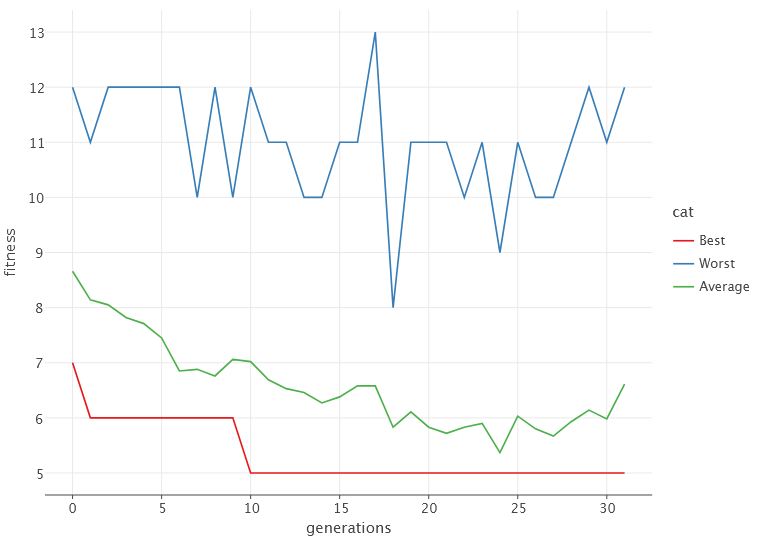
\includegraphics[width=0.6\textwidth]{img/java_6eGIGC5z5r.png}
  \caption{Evolution plot for the \textit{Room Scheduling} problem.}
  \label{fig:app:keen_room_scheduling}
\end{figure}
